% Texto opcional de integração: resultados publicados C07, apenas descrição.
\subsection{Descrição pareada das 500 realizações já publicadas}
\label{sec:comp-c07-descritivo}

A síntese publicada no capítulo~\ref{chap:validacao} permite descrever,
sem uma nova inferência, os contrastes A\_CN--A0\_CN, B\_CN--A\_CN e
B\_G--A\_G nos mesmos 500 dados. Nesta seção, a direção é sempre a
análise nova menos a anterior. Foram conferidos os 2.500 alvos, as 500
verdades originais e a identidade dos dados, prioris e arquivos publicados.
Todos os casos permanecem no resumo, inclusive aqueles com pendências
numéricas. A Tabela~\ref{tab:comp-descritivo500} mostra duas medidas de
posição das diferenças calculadas para a massa adimensional.

\begin{table}[htbp]
\centering\small
\caption{Descrição dos 500 valores pareados em unidades da largura da priori.
As médias e medianas não possuem aqui uma precisão horizontal certificada
dos quantis nem um intervalo de confiança associado.}
\label{tab:comp-descritivo500}
\begin{tabular}{lrrrr}
\toprule
Contraste & Média $\Delta Q_{95}(u)$ & Mediana & Média $\Delta W_{90}(u)$ & Mediana\\
\midrule
A\_CN$-$A0\_CN & 0,00130 & 0,00059 & $-0,00244$ & $-0,00007$\\
B\_CN$-$A\_CN & 0,00540 & $-0,00127$ & 0,01147 & 0,00213\\
B\_G$-$A\_G & 0,00477 & $-0,00061$ & 0,00652 & 0,00137\\
\bottomrule
\end{tabular}
\end{table}

As diferenças de quantis e de larguras são computadas por dado antes de
qualquer média ou mediana. Em dois contrastes, a média e a mediana de
$\Delta Q_{95}(u)$ têm sinais distintos. Esse fato limita a interpretação
da média isolada; não determina a direção de um deslocamento para cada
realização. A descrição completa retém os 20 quantis e as cinco larguras
centrais de 90\%, com as guardas por função preservadas em arquivos.

Os bins fixos $u\in[0;0{,}5),[0{,}5;0{,}9),[0{,}9;1]$ contêm
243, 208 e 49 dados; os bins $\gamma\in[3;4{,}25),[4{,}25;5{,}5]$
contêm 233 e 267 dados. As subdivisões se baseiam nas verdades e não
selecionam realizações pelo resultado das guardas. Percentis entre os casos,
quando apresentados nos arquivos, descrevem essa distribuição empírica;
não são intervalos de confiança da média. Pequenas diferenças ou
proximidade entre curvas não são convertidas em decisões de equivalência,
materialidade ou viés populacional. A análise inferencial pareada C08, com
brackets e incerteza explicitamente avaliados, permanece separada.

\begin{figure}[htbp]
 \centering
 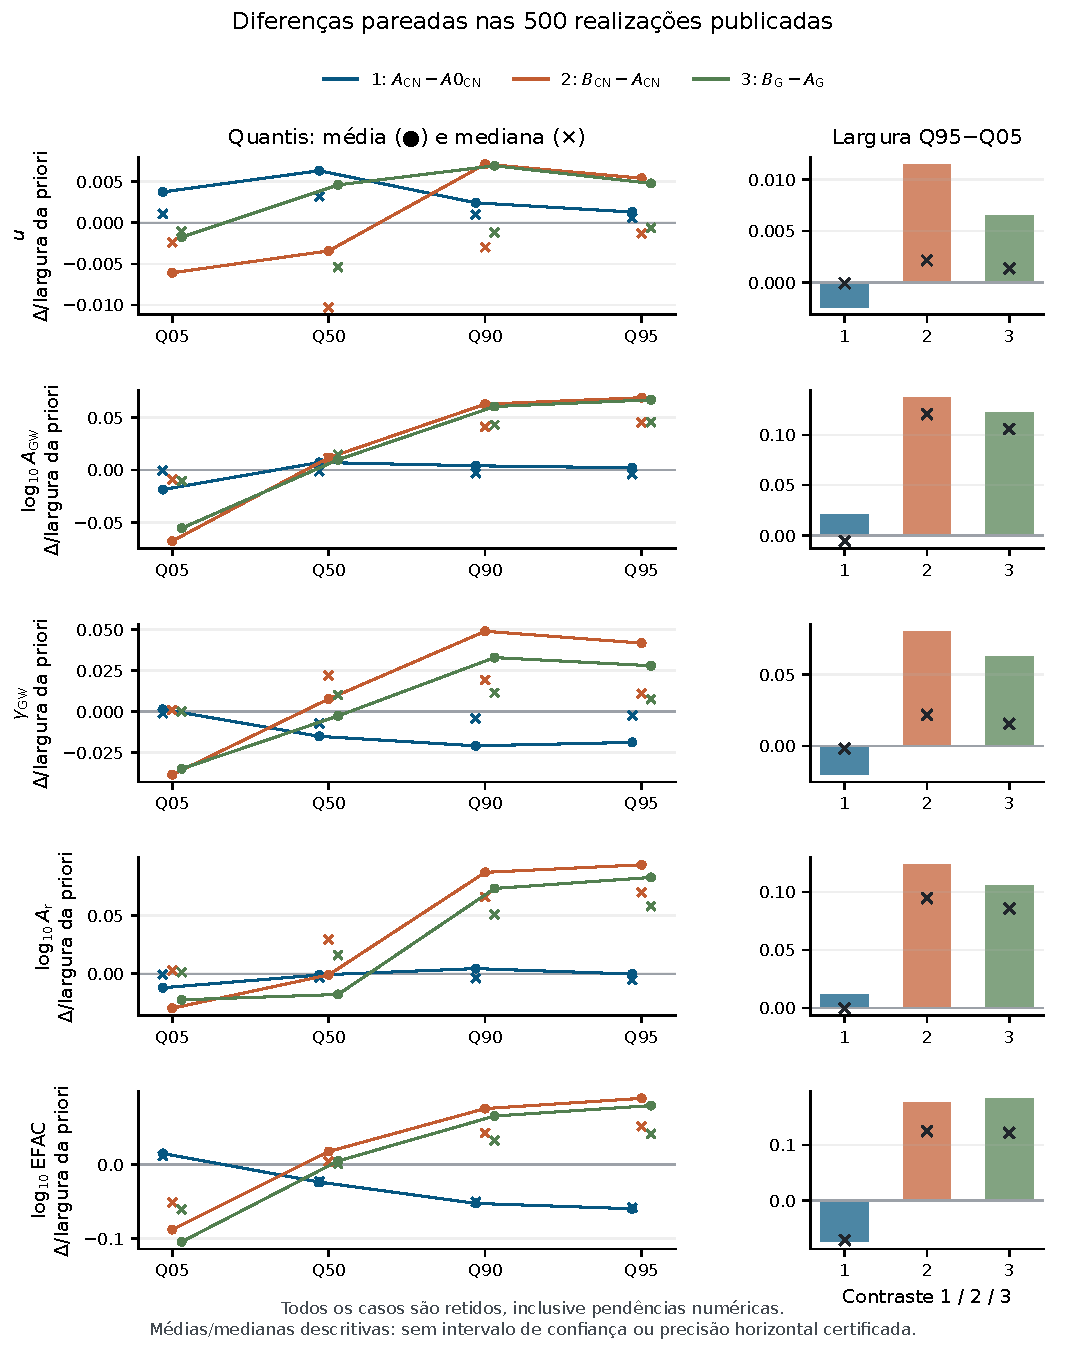
\includegraphics[width=\textwidth,height=.80\textheight,keepaspectratio]{../figures/compressao/c07_descritivo/paired_quantiles_widths.pdf}
 \caption{Médias e medianas descritivas das diferenças pareadas nos 500 dados
 publicados. A largura central é $W_{90}=Q_{95}-Q_{05}$. Todos os casos são
 retidos; a figura não contém barras de erro numérico ou intervalos de confiança.}
 \label{fig:comp-c07-pares}
\end{figure}

\begin{figure}[htbp]
 \centering
 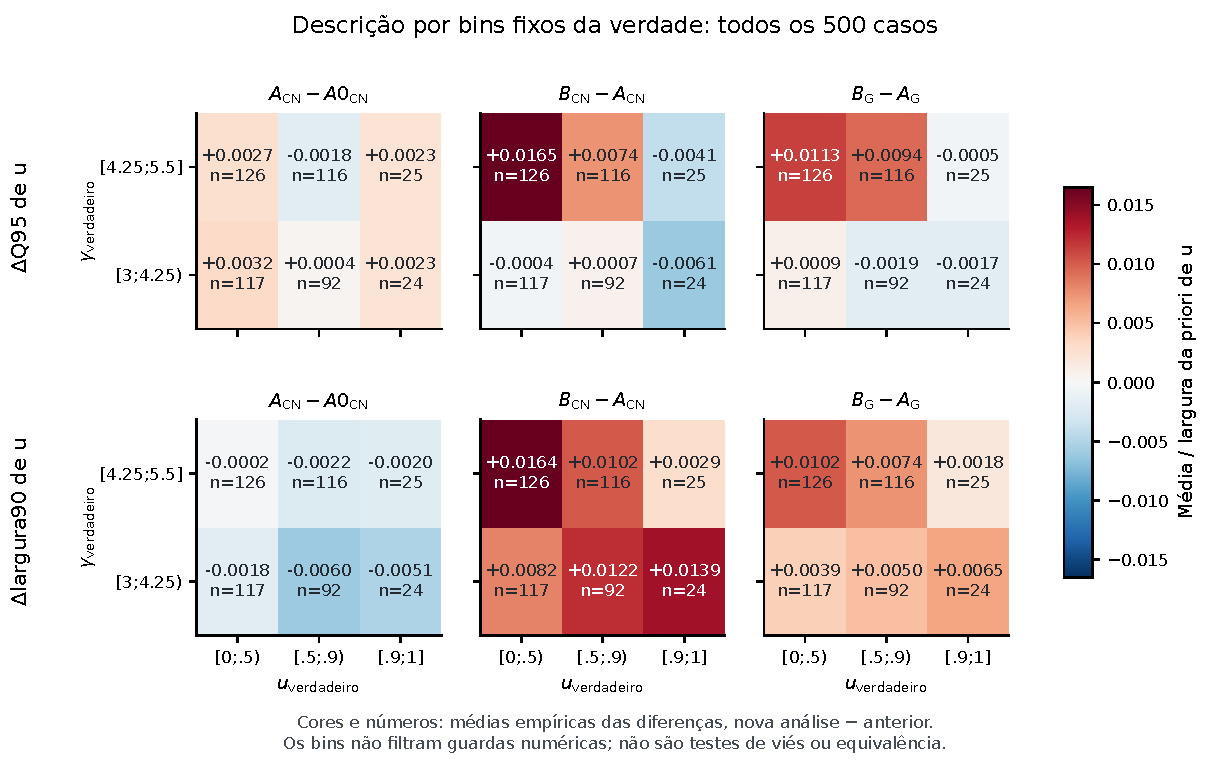
\includegraphics[width=\textwidth]{../figures/compressao/c07_descritivo/paired_mass_bins.pdf}
 \caption{Médias descritivas de $\Delta Q_{95}(u)$ e $\Delta W_{90}(u)$
 nos bins fixos da verdade. Cada célula informa seu número de dados;
 as pendências numéricas permanecem no denominador. As cores não expressam
 significância estatística nem equivalência entre as análises.}
 \label{fig:comp-c07-bins}
\end{figure}
